\documentclass[conference]{IEEEtran}
\IEEEoverridecommandlockouts
\usepackage{cite}
\usepackage{amsmath,amssymb,amsthm}
\usepackage{booktabs}
\usepackage{graphicx}
\usepackage{xcolor}
\usepackage{colortbl}
\usepackage{algorithm}
\usepackage{algpseudocode}
\usepackage{tikz}
\usetikzlibrary{positioning,shapes.geometric,arrows.meta,fit,calc,backgrounds,patterns}
\usepackage{pgfplots}
\usepgfplotslibrary{polar}
\pgfplotsset{compat=1.16}
\usepackage[hidelinks]{hyperref}
\newtheorem{proposition}{Proposition}

% Set to \extendedtrue after the extra questions have been run and Table~\ref{tab:extended} is filled in.
\newif\ifextended
\extendedfalse

\begin{document}

\title{Agreement-Gated Visual Adjudication for\\Long Visual Document Question Answering}

\author{\IEEEauthorblockN{Mariam Zahid}
\IEEEauthorblockA{\textit{Artificial Intelligence, Fast NUCES}\\
Islamabad, Pakistan}}

\maketitle

\begin{abstract}
Long visual document question answering systems first find the evidence pages, then sample several candidate answers, and finally let an Adjudicator choose one. In DocLens, this last step runs on every question and reads only the text of the candidates, although the sampled answers already agree on about half of the questions. We study when adjudication is needed and what the Adjudicator should see. We propose gated visual adjudication. An agreement gate skips the Adjudicator when all $k$ sampled answers agree, and otherwise a visual Adjudicator checks the candidates against the evidence pages. We formalize the pipeline, derive the accuracy change and the token cost of the gate, and show when a gate is lossless. With Qwen3-VL-8B on 200 MMLongBench-Doc questions, the method calls the Adjudicator on 52\% of the questions instead of all of them and raises the accuracy from 56.3\% to 57.3\%, with gains on table (+5.0) and figure (+2.0) questions, at 6.7\% more tokens. The improvement lies within the sampling error of 200 questions. The agreement of the samples predicts when adjudication helps, and most remaining errors come from evidence retrieval and reading, not from the final decision.
\end{abstract}

\begin{IEEEkeywords}
document question answering, long documents, multi-agent systems, adjudication, agreement gate, vision-language models
\end{IEEEkeywords}

% Paper body shared by main.tex (IEEEtran) and sn-article.tex (Springer Nature).
% Needs, from the wrapper: \ifextended, the proposition environment, and the algorithm packages.

\section{Introduction}
\label{sec:intro}

Reports, manuals and research papers contain text, tables, charts and figures, and they often have dozens of pages. Visual document understanding (VDU) is the task of reading such documents the way a person does. A VDU system has to read the words, the layout and the images together \cite{xu2020layoutlm,kim2022donut}. A common VDU task is visual question answering (VQA): the system gets an image and a question in natural language and returns an answer \cite{antol2015vqa}. When the image is a document page, the task is called DocVQA \cite{mathew2021docvqa}. The task matters in daily work. A worker needs one number from a financial report, a student needs one result from a paper, and a technician needs one step from a long manual. A wrong answer can cost money or cause harm, so a system must be both fast and correct.

Long documents make the task much harder. The evidence for a question can be a table on one page and a chart on another, and about a quarter of the questions in MMLongBench-Doc cannot be answered from the document at all \cite{ma2024mmlongbench}. The best vision-language models (VLMs) still make many mistakes on this benchmark \cite{ma2024mmlongbench,comanici2025gemini}. A system has to solve two problems: it must find the pages and the page elements that hold the evidence, and it must turn this evidence into one correct answer.

Recent systems split the work between several steps or agents \cite{zhu2025doclens,jain2025simpledoc,han2025mdocagent,slideagent,orca,docvstar}. DocLens \cite{zhu2025doclens} is a strong example. Its Lens Module finds the evidence pages and crops tables and figures from them. Its Reasoning Module then samples several candidate answers with an Answer Sampler, and an Adjudicator reads the candidates and chooses the final answer. DocLens reaches 67.6\% accuracy on MMLongBench-Doc with Gemini-2.5-Pro and 61.1\% with Qwen3-VL-8B on a sample of 200 questions \cite{zhu2025doclens}. Its own ablation shows that the whole Reasoning Module adds only 0.6 points for Gemini-2.5-Pro (67.0 without it, 67.6 with it) \cite{zhu2025doclens}. This raises a question about the last step: how much does the Adjudicator add, and when does it add it?

The Adjudicator has three weaknesses. It runs on every question, so it adds one more model call everywhere. It reads only the text of the candidate analyses and answers, and it does not see the document pages, so it cannot check the candidates against the evidence. And it can overturn an answer that was already correct. ORCA reports the same effect for its verification stages: 12\% of 100 analyzed failures are over-refinement, where a later stage overrides a correct answer, and ORCA skips its debate stages when two agents agree, which happens in 77\% of its cases \cite{orca}. In our reproduction of DocLens with Qwen3-VL-8B, the eight sampled answers agree on 48\% of the questions, the text-only Adjudicator and the majority vote give a different score on only 4.5\% of the questions, and yet for 15.5\% of the questions a correct candidate exists but the final answer is wrong.

These facts suggest two changes. First, the Adjudicator is not needed when the candidates agree. Second, when they disagree, the Adjudicator should look at the pages. We propose gated visual adjudication. An agreement gate counts how many of the $k=8$ sampled answers agree and returns the majority answer when all of them agree. When they disagree, a visual Adjudicator reads the evidence pages together with the candidate answers and chooses one. The method needs no training and does not change the DocLens prompts for the Lens Module or the Answer Sampler. With Qwen3-VL-8B on 200 MMLongBench-Doc questions, it calls the Adjudicator on 52\% of the questions instead of all of them and raises the accuracy from 56.3\% to 57.3\%, with the largest gains on table and figure questions, at the price of 6.7\% more tokens. The gain is small, and we report its confidence interval. Our contributions are as follows.

\begin{itemize}
  \item We formalize the final decision step of sampling-based document agents. We derive the accuracy change and the token cost of an agreement gate and show when a gate is lossless (Section~\ref{sec:method}).
  \item We propose a visual Adjudicator that conditions on the evidence pages and chooses among the candidate answers, and we use it behind a unanimity gate.
  \item We reproduce vanilla Qwen3-VL-8B, Qwen3-VL-8B with OCR and DocLens on a seeded sample of 200 MMLongBench-Doc questions, compare with published results, and analyze how sample agreement predicts when adjudication helps (Section~\ref{sec:experiments}).
\end{itemize}

\section{Related Work}
\label{sec:related}

Early work on document images combined OCR text with the position of each word. LayoutLM learns from text and layout together \cite{xu2020layoutlm}, and Donut reads the page image without OCR \cite{kim2022donut}. Single-page question answering datasets cover forms and scans (DocVQA \cite{mathew2021docvqa}), infographics \cite{mathew2022infographicvqa}, charts \cite{masry2022chartqa} and slides \cite{tanaka2023slidevqa}. Multi-page datasets followed: MP-DocVQA \cite{tito2023mpdocvqa}, DUDE \cite{vanlandeghem2023dude}, DocBench \cite{zou2024docbench}, LongDocURL \cite{deng2025longdocurl} and MMLongBench-Doc \cite{ma2024mmlongbench}, which also contains unanswerable questions. Open vision-language models such as Qwen2.5-VL and Qwen3-VL \cite{bai2025qwen25vl,bai2025qwen3vl} and proprietary models \cite{hurst2024gpt4o,comanici2025gemini} read page images directly, but they lose small details when many pages are given at once.

A first line of work retrieves pages before answering. ColBERT-style and ColPali retrievers score pages with late interaction \cite{santhanam2022colbertv2,faysse2024colpali}, and VisRAG, VDocRAG and M3DocRAG feed the retrieved page images to a VLM \cite{yu2024visrag,tanaka2025vdocrag,cho2024m3docrag}, in the spirit of retrieval-augmented generation \cite{lewis2020rag}. MMDocIR studies retrieval for long documents \cite{dong2025mmdocir}. A second line uses several agents or steps, in the spirit of agents that reason and act \cite{yao2023react}. MDocAgent combines text and image agents \cite{han2025mdocagent}, MACT uses collaborating agents with test-time scaling \cite{yu2025mact}, SimpleDoc retrieves pages and refines the query in several rounds \cite{jain2025simpledoc}, SlideAgent uses global, page and element agents \cite{slideagent}, and ORCA adds routing, debate and answer refinement \cite{orca}. Doc-V* trains a navigation agent with imitation and reinforcement learning \cite{docvstar}. DocLens finds pages with OCR-augmented VLMs, crops page elements, and chooses among sampled answers with an Adjudicator \cite{zhu2025doclens}. These works mostly improve where the evidence is found or how agents cooperate. We study the last step, the choice among candidate answers.

Sampling several answers and combining them is a standard way to reduce errors. Self-consistency takes the most frequent answer among sampled reasoning paths \cite{wang2023selfconsistency}, which builds on chain-of-thought prompting \cite{wei2022cot}. Language models can also judge answers \cite{zheng2023judging} or debate them \cite{du2024debate}, but models that revise their own answers without outside information can make them worse \cite{huang2024selfcorrect}. Our over-correction measure captures this effect. Deciding when to run a costly step is related to selective prediction, where a classifier abstains below a confidence threshold \cite{geifman2017selective}, to confidence calibration \cite{guo2017calibration}, and to model cascades that call an expensive model only when needed \cite{chen2024frugalgpt}. We use the agreement of the samples as the confidence signal.

\section{Problem Formulation}
\label{sec:formulation}

A document is a sequence of pages $D=(p_1,\dots,p_N)$. From each page $p_j$ we obtain its screenshot, its extracted text $t_j$ and a set of cropped visual elements $V_j$ (tables, figures and charts). Given a question $q$, the goal is to return an answer $\hat y$ that matches the reference answer $y^\ast$. Following DocLens \cite{zhu2025doclens}, we factor the answering function into evidence extraction, answer sampling and a final decision. The Lens Module $\mathcal{L}$ extracts the evidence
\begin{equation}
E=\mathcal{L}(D,q)=\{(p_j,t_j,V_j)\}_{j\in P},\qquad P\subseteq\{1,\dots,N\},
\label{eq:lens}
\end{equation}
where $P$ is the set of pages found by the Page Navigator. The Answer Sampler draws $k$ reasoning--answer pairs from the backbone $\pi_\theta$ at temperature $T$,
\begin{equation}
(r_i,y_i)\sim\pi_\theta(\,\cdot\mid q,E\,),\qquad i=1,\dots,k.
\label{eq:sampler}
\end{equation}
A final decision function $\Phi$ maps the question, the evidence and the candidates to the answer,
\begin{equation}
\hat y=\Phi\bigl(q,E,\{(r_i,y_i)\}_{i=1}^{k}\bigr).
\label{eq:decision}
\end{equation}
DocLens uses a text-only Adjudicator $\mathcal{A}_{\mathrm{text}}(q,\{(r_i,y_i)\})$ for $\Phi$, which ignores $E$ and runs on every question. Let $s(\hat y,y^\ast)\in[0,1]$ be the official benchmark score, which gives partial credit for list answers. The accuracy of a decision function is
\begin{equation}
\mathrm{Acc}(\Phi)=\frac{1}{M}\sum_{m=1}^{M}s\bigl(\Phi(q_m,E_m,\{(r_i,y_i)\}_m),\,y^\ast_m\bigr)
\label{eq:acc}
\end{equation}
over $M$ questions. The cost $C(\Phi)$ is the number of tokens spent per question, summed over all steps. We look for a $\Phi$ with high $\mathrm{Acc}(\Phi)$ and low $C(\Phi)$, without training and without changing $\mathcal{L}$ and $\pi_\theta$.

\section{Gated Visual Adjudication}
\label{sec:method}

Figure~\ref{fig:pipeline} shows the pipeline. The Lens Module and the Answer Sampler are those of DocLens. We change only the decision step $\Phi$ of Eq.~\eqref{eq:decision}.

\begin{figure*}[t]
\centering
\resizebox{0.96\textwidth}{!}{%
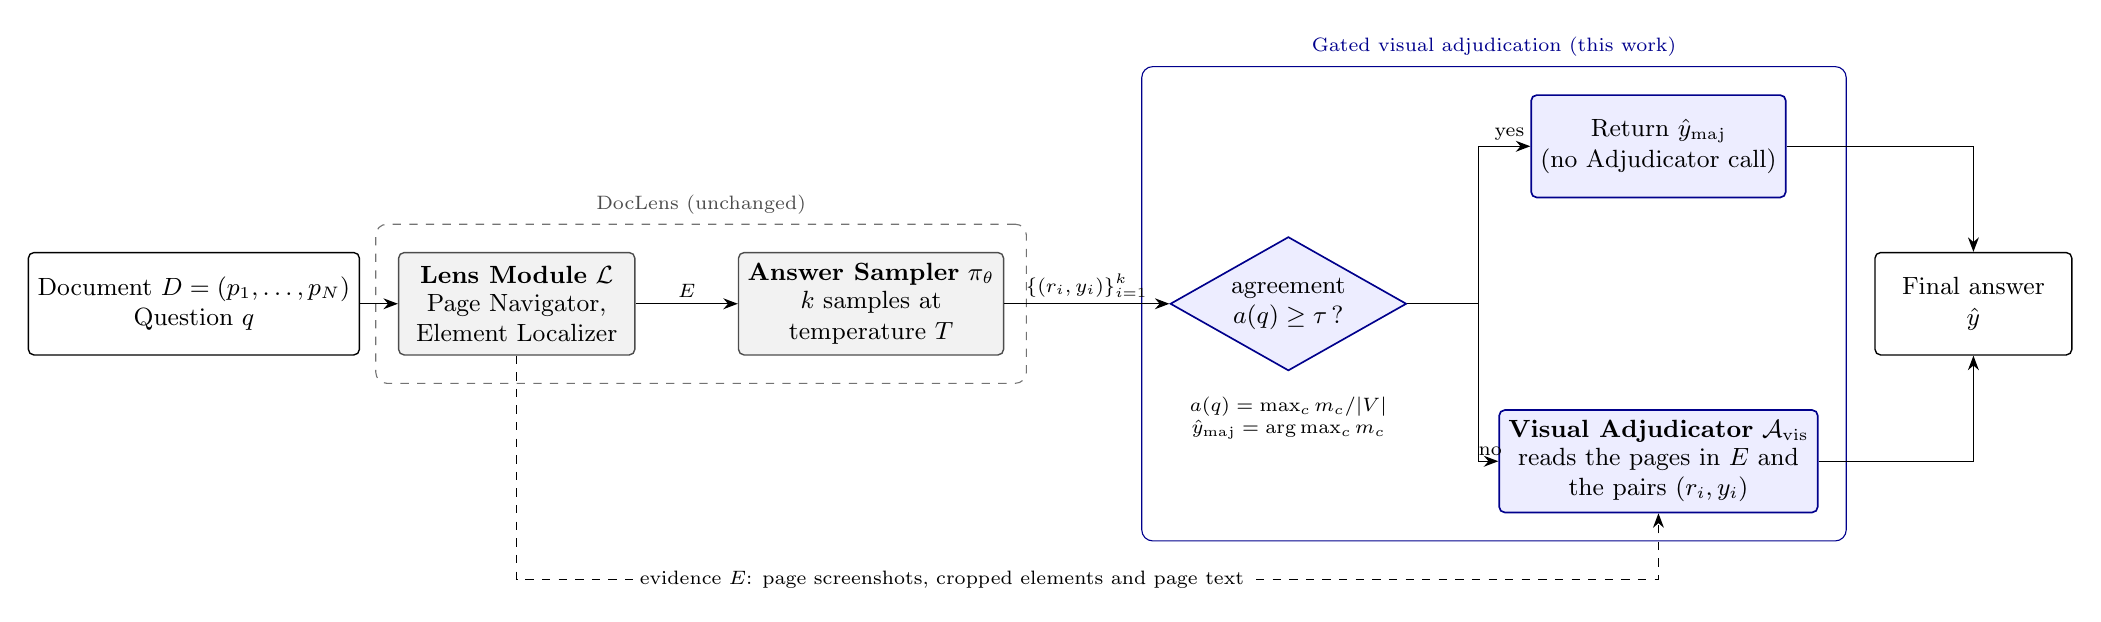
\begin{tikzpicture}[
  font=\small,
  >=Stealth,
  io/.style={draw, rounded corners=2pt, minimum height=1.3cm, minimum width=2.5cm, align=center, fill=white, line width=0.5pt},
  old/.style={draw=black!70, rounded corners=2pt, minimum height=1.3cm, minimum width=3.0cm, align=center, fill=black!5, line width=0.5pt},
  new/.style={draw=blue!55!black, rounded corners=2pt, minimum height=1.3cm, minimum width=3.1cm, align=center, fill=blue!7, line width=0.6pt},
  gate/.style={draw=blue!55!black, diamond, aspect=1.9, inner sep=0pt, align=center, fill=blue!7, line width=0.6pt},
  arr/.style={->, line width=0.5pt},
  lab/.style={font=\scriptsize, inner sep=2pt}
]
\node[io] (in) at (0,0) {Document $D=(p_1,\dots,p_N)$\\Question $q$};
\node[old] (lens) at (4.1,0) {\textbf{Lens Module} $\mathcal{L}$\\[-1pt] Page Navigator,\\Element Localizer};
\node[old] (samp) at (8.6,0) {\textbf{Answer Sampler} $\pi_\theta$\\[-1pt] $k$ samples at\\temperature $T$};
\node[gate, minimum width=3.0cm, minimum height=1.7cm] (g) at (13.9,0) {agreement\\$a(q)\ge\tau$\,?};
\node[new] (maj) at (18.6,2.0) {Return $\hat y_{\mathrm{maj}}$\\(no Adjudicator call)};
\node[new] (vis) at (18.6,-2.0) {\textbf{Visual Adjudicator} $\mathcal{A}_{\mathrm{vis}}$\\[-1pt] reads the pages in $E$ and\\the pairs $(r_i,y_i)$};
\node[io] (out) at (22.6,0) {Final answer\\$\hat y$};
\node[lab, align=center] (def) at (13.9,-1.45) {$a(q)=\max_c m_c/|V|$\\$\hat y_{\mathrm{maj}}=\arg\max_c m_c$};
\draw[arr] (in) -- (lens);
\draw[arr] (lens) -- node[lab, above] {$E$} (samp);
\draw[arr] (samp) -- node[lab, above] {$\{(r_i,y_i)\}_{i=1}^{k}$} (g);
\draw[arr] (g.east) -- ++(0.9,0) |- node[lab, pos=0.8, above] {yes} (maj.west);
\draw[arr] (g.east) -- ++(0.9,0) |- node[lab, pos=0.8, above] {no} (vis.west);
\draw[arr] (maj.east) -| (out.north);
\draw[arr] (vis.east) -| (out.south);
\draw[arr, dashed] (lens.south) -- (4.1,-3.5) -- (18.6,-3.5) -- (vis.south);
\node[lab, fill=white] at (9.5,-3.5) {evidence $E$: page screenshots, cropped elements and page text};
\begin{scope}[on background layer]
 \node[draw=black!55, dashed, rounded corners=4pt, fit=(lens)(samp), inner xsep=8pt, inner ysep=10pt, label={[font=\scriptsize, text=black!70]above:DocLens (unchanged)}] {};
 \node[draw=blue!55!black, rounded corners=4pt, fit=(g)(maj)(vis), inner xsep=10pt, inner ysep=10pt, label={[font=\scriptsize, text=blue!55!black]above:Gated visual adjudication (this work)}] {};
\end{scope}
\end{tikzpicture}}
\caption{Pipeline of gated visual adjudication. The Lens Module and the Answer Sampler are those of DocLens (Eqs.~\eqref{eq:lens} and \eqref{eq:sampler}). The agreement $a(q)$ of the $k$ sampled answers (Eq.~\eqref{eq:agreement}) decides whether the majority answer is returned or the visual Adjudicator (Eq.~\eqref{eq:visual}) is called. Our additions are shaded blue.}
\label{fig:pipeline}
\end{figure*}

\subsection{Agreement Gate}
Let $n(\cdot)$ be a normalization that lower-cases an answer and removes spaces and punctuation. Let $V=\{i: n(y_i)\notin\{\emptyset,\text{error}\}\}$ be the valid candidates, and let $m_c=|\{i\in V:n(y_i)=c\}|$ count the candidates that equal the normalized answer $c$. The majority answer and the agreement of the question are
\begin{equation}
\hat y_{\mathrm{maj}}=\arg\max_c m_c,\qquad a(q)=\frac{\max_c m_c}{|V|}\in\Bigl[\tfrac{1}{|V|},1\Bigr],
\label{eq:agreement}
\end{equation}
with $a(q)=0$ when $V=\emptyset$. The gate returns the majority answer when the agreement reaches a threshold $\tau$, and calls an adjudicator otherwise:
\begin{equation}
\Phi_\tau(q)=
\begin{cases}
\hat y_{\mathrm{maj}} & \text{if } a(q)\ge\tau,\\[2pt]
\mathcal{A}\bigl(q,E,\{(r_i,y_i)\}_{i=1}^{k}\bigr) & \text{otherwise.}
\end{cases}
\label{eq:gate}
\end{equation}
In our main setting $\tau=1$: the adjudicator is skipped only when all valid candidates agree. This rule is fixed in advance and has no tuned parameter. Section~\ref{sec:experiments} also tests thresholds chosen on the data.

\subsection{Visual Adjudicator}
The text-only Adjudicator of DocLens decides from the written analyses alone. Our visual Adjudicator $\mathcal{A}_{\mathrm{vis}}$ also receives the evidence $E$, which are the page screenshots, the cropped elements and the page text that the Answer Sampler saw:
\begin{equation}
\hat y=\mathcal{A}_{\mathrm{vis}}\bigl(q,E,\{(r_i,y_i)\}_{i=1}^{k}\bigr)\in\{y_1,\dots,y_k\}\cup\{\bot\},
\label{eq:visual}
\end{equation}
where $\bot$ stands for the answer ``Not answerable''. It uses the same backbone, so there are no new parameters. Its prompt is the DocLens Adjudicator prompt with two additions: the model must check the values that the competing answers depend on against the page images, and it must choose the text of one candidate instead of writing a new answer, or answer ``Not answerable'' when the pages do not contain the requested value. Each analysis is cut to 2,000 characters, the temperature is 0, and if the output cannot be parsed, we return the DocLens answer. Algorithm~\ref{alg:gva} gives the complete procedure.

\begin{algorithm}[t]
\caption{Gated visual adjudication for one question}
\label{alg:gva}
\begin{algorithmic}[1]
\Require document $D$, question $q$, samples $k$, threshold $\tau$
\State $E\gets\mathcal{L}(D,q)$ \Comment{Lens Module}
\State draw $(r_i,y_i)\sim\pi_\theta(\cdot\mid q,E)$, $i=1,\dots,k$ \Comment{sampler}
\State compute $V$, $\hat y_{\mathrm{maj}}$ and $a(q)$ by Eq.~\eqref{eq:agreement}
\If{$a(q)\ge\tau$}
  \State \Return $\hat y_{\mathrm{maj}}$ \Comment{no call}
\Else
  \State \Return $\mathcal{A}_{\mathrm{vis}}(q,E,\{(r_i,y_i)\}_{i=1}^{k})$
\EndIf
\end{algorithmic}
\end{algorithm}

\subsection{Accuracy and Cost of the Gate}
Let $G_\tau=\{q: a(q)\ge\tau\}$ be the questions that the gate answers itself and $p=\Pr[q\in G_\tau]$ the skipped fraction. Let $\Phi_{\mathcal{A}}$ be the pipeline that always runs the adjudicator $\mathcal{A}$.

\begin{proposition}
\label{prop:acc}
For the same adjudicator $\mathcal{A}$,
\[
\mathrm{Acc}(\Phi_\tau)-\mathrm{Acc}(\Phi_{\mathcal{A}})=\frac{1}{M}\sum_{q\in G_\tau}\Bigl[s(\hat y_{\mathrm{maj}},y^\ast)-s\bigl(\mathcal{A}(q),y^\ast\bigr)\Bigr].
\]
\end{proposition}
\begin{proof}
The two pipelines return the same answer for every question outside $G_\tau$, so only the questions in $G_\tau$ contribute to the difference.
\end{proof}

The difference is the number of over-corrections avoided minus the number of fixes lost on $G_\tau$. For $\tau=1$ and the text-only Adjudicator, it is zero whenever the Adjudicator returns the shared answer on unanimous questions, and we measure exactly this in Section~\ref{sec:experiments}.

\begin{proposition}
\label{prop:cost}
Let $C_0$ be the tokens spent by $\mathcal{L}$ and the sampler, and $C_{\mathcal{A}}$ the tokens of one adjudicator call. The expected cost is $C(\Phi_\tau)=C_0+(1-p)\,C_{\mathcal{A}}$, so the gate saves $p\,C_{\mathcal{A}}$ per question. Compared with always running the text-only Adjudicator (cost $C_{\mathrm{text}}$), a visual Adjudicator (cost $C_{\mathrm{vis}}$) behind the gate does not increase the cost if and only if $p\ge 1-C_{\mathrm{text}}/C_{\mathrm{vis}}$.
\end{proposition}
\begin{proof}
The adjudicator is called with probability $1-p$, which gives the expected cost. The condition follows from $(1-p)C_{\mathrm{vis}}\le C_{\mathrm{text}}$.
\end{proof}

Two bounds limit what any selection among the candidates can do. No decision function that only selects among the candidates can exceed $\mathrm{pass@}k=\frac{1}{M}\sum_m\max_i s(y_i,y^\ast_m)$, and a gate over $\hat y_{\mathrm{maj}}$ and $\mathcal{A}_{\mathrm{text}}$ cannot exceed the oracle that picks the better of the two answers for each question.

\section{Experiments}
\label{sec:experiments}

\subsection{Experimental Setup}
We use MMLongBench-Doc \cite{ma2024mmlongbench}, with 1,082 questions on long PDF documents of 49.4 pages on average. Each question has an evidence source (text, layout, chart, table or figure), and 22.8\% of the questions have no answer in the document. The original DocLens evaluation of Qwen3-VL-8B uses a random sample of 200 questions that is not published \cite{zhu2025doclens}, so we draw our own sample of 200 questions with a fixed seed. It covers 95 documents and is the same for every method.

We compare vanilla Qwen3-VL-8B (screenshots only), Qwen3-VL-8B with OCR text, DocLens, majority voting over the eight samples, the gate with the text-only Adjudicator ($\tau=1$ and a threshold chosen by five-fold cross-validation over documents), and our gated visual Adjudicator. All methods use Qwen3-VL-8B-Instruct served with vLLM \cite{kwon2023vllm} on two NVIDIA T4 GPUs, with the DocLens settings $k=8$ and $T=0.7$ and page text from MinerU \cite{wang2024mineru}. The memory of the T4 GPUs limits the context to 40,960 tokens. The Page Navigator therefore reads documents in chunks of six pages, images are halved when a prompt is too long, and answers are extracted for scoring with the same Qwen model instead of Gemini-2.5-Flash. We report accuracy under the official scoring (Eq.~\eqref{eq:acc}) and four further measures. The Adjudicator rate is $\frac{1}{M}\sum_m\mathbb{1}[a(q_m)<\tau]$. With $\hat y_m$ the returned answer and a score of at least 0.5 counted as correct, the over-correction rate and the fix rate are
\begin{equation}
\begin{aligned}
\mathrm{OC}&=\tfrac{1}{M}\textstyle\sum_m\mathbb{1}\bigl[s(\hat y_{\mathrm{maj},m},y^\ast_m)\ge0.5,\; s(\hat y_m,y^\ast_m)<0.5\bigr],\\
\mathrm{Fix}&=\tfrac{1}{M}\textstyle\sum_m\mathbb{1}\bigl[s(\hat y_{\mathrm{maj},m},y^\ast_m)<0.5,\; s(\hat y_m,y^\ast_m)\ge0.5\bigr],
\end{aligned}
\label{eq:ocfix}
\end{equation}
so that Proposition~\ref{prop:acc} states that gating changes the accuracy by the difference of the two rates on the skipped questions. The fourth measure is the number of tokens per question. For the difference $\Delta=\mathrm{Acc}(\Phi_1)-\mathrm{Acc}(\Phi_2)$ of two methods, we resample the $M$ questions with replacement 10,000 times, recompute $\Delta$ on each resample, and report the 2.5th and 97.5th percentiles as the 95\% confidence interval \cite{efron1979bootstrap,berg2012empirical}.

\subsection{Main Results}
Table~\ref{tab:literature} places our results next to published ones on MMLongBench-Doc. The numbers of the other methods are copied from the cited papers, with different backbones and different evaluation samples, so the table shows the landscape and not a controlled comparison. The two rows that are directly comparable are the DocLens numbers with Qwen3-VL-8B. Our reproduction reaches 56.3\% against the published 61.1\% and our vanilla and OCR baselines reach 40.9\% and 37.3\% against 43.0\% and 42.9\% (Table~\ref{tab:ours}). The gap has several likely causes: the shorter context of the T4 setup, the Qwen answer extractor, and a lower page recall of our Page Navigator (88.4\% against 97.3\% for Gemini-2.5-Pro in the DocLens paper). OCR text is worse than screenshots alone in our setup, while the original paper reports almost equal values, which we attribute to the longer prompts that OCR text creates.

\begin{table}[t]
\caption{Accuracy (\%) on MMLongBench-Doc of published methods and ours. Values are copied from the cited papers (the SimpleDoc and screenshots-plus-OCR values are from the DocLens paper, which reproduced them); backbones and evaluation samples differ. Rows marked $^\ddagger$ use a random sample of 200 questions (our own sample for the last two rows). Human experts reach 65.8.}
\label{tab:literature}
\centering
\footnotesize
\begin{tabular}{@{}llc@{}}
\toprule
Method & Backbone & Acc. \\
\midrule
GPT-4o \cite{ma2024mmlongbench} & GPT-4o & 42.8 \\
Screenshots + OCR \cite{zhu2025doclens} & Gemini-2.5-Pro & 63.3 \\
M3DocRAG \cite{cho2024m3docrag} & Qwen2-VL-7B & 21.0 \\
MDocAgent \cite{han2025mdocagent} & GPT-4o & 42.0 \\
Doc-V* \cite{docvstar} & Qwen2.5-VL-7B & 42.1 \\
MACT \cite{yu2025mact} & MiMo-VL-7B & 47.4 \\
SimpleDoc \cite{jain2025simpledoc,zhu2025doclens} & Claude-4-Sonnet & 58.6 \\
DocLens \cite{zhu2025doclens} & Gemini-2.5-Pro & 67.6 \\
DocLens \cite{zhu2025doclens}$^\ddagger$ & Qwen3-VL-8B & 61.1 \\
\midrule
DocLens, our reproduction$^\ddagger$ & Qwen3-VL-8B & 56.3 \\
Gated visual adjudication (ours)$^\ddagger$ & Qwen3-VL-8B & 57.3 \\
\bottomrule
\end{tabular}
\end{table}

Table~\ref{tab:ours} gives the controlled comparison on our sample. Majority voting without any Adjudicator is 1.5 points below DocLens. The gate with $\tau=1$ and the text-only Adjudicator keeps the accuracy of DocLens (56.3) and removes 48\% of the Adjudicator calls, but it saves only 1.1\% of the tokens, because the text-only Adjudicator uses about 2,600 of the 87,620 tokens of a question (3\%) and the Lens Module uses about 70,000. A threshold chosen by cross-validation (0.875, 0.75, 0.875, 0.375 and 0.875 in the five folds) is worse (54.8). The gated visual Adjudicator reaches 57.3, which is 1.0 point above DocLens and 2.5 points above majority voting. The 95\% confidence interval of the gain over DocLens is $-2.5$ to $+4.5$ points, and the interval of the gain over majority voting is $-0.5$ to $+5.9$ points, so a sample of 200 questions cannot separate the methods. On the 104 questions where the answers disagree, the accuracy rises from 36.9 to 38.8: the visual Adjudicator fixes 7 questions that DocLens answers wrongly and breaks 5 that DocLens answers correctly. The visual Adjudicator is more expensive. By Proposition~\ref{prop:cost}, one visual call costs about $C_{\mathrm{vis}}\approx16{,}300$ tokens against $C_{\mathrm{text}}\approx2{,}600$ for a text-only call, so the visual Adjudicator is token-neutral only if the gate skips at least $1-C_{\mathrm{text}}/C_{\mathrm{vis}}\approx84\%$ of the questions. Our gate skips 48\%, and the total cost rises by 6.7\%.

\begin{table}[t]
\caption{Results on our 200 questions with Qwen3-VL-8B. Over-correction (OC) and fix rate (Fix) are not defined for the baselines without an Adjudicator. Tokens are per question.}
\label{tab:ours}
\centering
\footnotesize
\setlength{\tabcolsep}{3.5pt}
\begin{tabular}{@{}lccccc@{}}
\toprule
Method & Acc. & OC / Fix & Adjud. & Tokens & $\Delta$ vs.\ DocLens \\
\midrule
Vanilla & 40.9 & -- & -- & -- & $-15.4$ \\
Vanilla + OCR & 37.3 & -- & -- & -- & $-19.0$ \\
Majority vote & 54.8 & 0.0 / 0.0 & 0\% & 84,977 & $-1.5$ \\
DocLens & 56.3 & 1.5 / 3.0 & 100\% & 87,620 & -- \\
Gate, CV threshold & 54.8 & 1.5 / 1.5 & 30\% & 85,940 & $-1.5$ \\
Gate, $\tau=1$, text-only & 56.3 & 1.5 / 3.0 & 52\% & 86,649 & $0.0$ \\
Gate + visual (ours) & 57.3 & -- & 52\% & 93,456 & $+1.0$ \\
\bottomrule
\end{tabular}
\end{table}

Table~\ref{tab:tokens} shows where the tokens go. The Lens Module dominates the cost, the text-only Adjudicator is cheap, and one visual call is about six times as expensive as a text-only call.

\begin{table}[t]
\caption{Tokens per question by stage for DocLens with Qwen3-VL-8B on our 200 questions. The last line is the cost of one visual Adjudicator call, computed from Table~\ref{tab:ours}.}
\label{tab:tokens}
\centering
\footnotesize
\begin{tabular}{@{}lcc@{}}
\toprule
Stage & Tokens & Share \\
\midrule
Lens Module & 70,200 & 80.1\% \\
Answer Sampler ($k=8$, one request) & 14,800 & 16.9\% \\
Text-only Adjudicator & 2,600 & 3.0\% \\
\midrule
Visual Adjudicator (one call) & 16,300 & -- \\
\bottomrule
\end{tabular}
\end{table}

Table~\ref{tab:cat} breaks the accuracy down by evidence source. The gain of our method is on table questions (+5.0) and figure questions (+2.0), where values must be read from the page image, and it is zero on text, layout and chart questions. Unanswerable questions lose 2.7 points, because the visual Adjudicator sometimes accepts a value that is close to the requested one. DocLens is much better than both baselines in every category, and most of all on unanswerable questions (75.7 against 45.0 for vanilla).

\begin{table*}[t]
\caption{Accuracy (\%) by evidence source on our 200 questions. TXT: plain text, LAY: layout, CHA: chart, TAB: table, FIG: figure, UNA: unanswerable, ANS: answerable. A question can have several evidence sources.}
\label{tab:cat}
\centering
\footnotesize
\begin{tabular}{@{}lcccccccc@{}}
\toprule
Method & TXT & LAY & CHA & TAB & FIG & UNA & ANS & All \\
\midrule
Vanilla & 38.1 & 47.3 & 30.3 & 36.7 & 47.5 & 45.0 & 40.0 & 40.9 \\
Vanilla + OCR & 32.8 & 24.0 & 20.8 & 27.3 & 38.1 & 56.8 & 32.9 & 37.3 \\
DocLens & 51.2 & 48.0 & 41.5 & 44.8 & 53.7 & 75.7 & 51.9 & 56.3 \\
Gated visual adjudication (ours) & 51.2 & 48.0 & 41.5 & 49.8 & 55.7 & 73.0 & 53.7 & 57.3 \\
\bottomrule
\end{tabular}
\end{table*}

\subsection{Analysis}
\vspace{3pt}\noindent\textit{Agreement predicts when adjudication helps.} Figure~\ref{fig:agreement} groups the questions by the agreement $a(q)$ of the eight samples. When all samples agree (48.0\% of the questions), the majority answer and the text-only Adjudicator have the same accuracy (77.3\%), so the gate loses nothing there, as Proposition~\ref{prop:acc} predicts. Accuracy falls quickly as agreement falls, and the Adjudicator is above the majority answer only on the disagreeing questions (by 2.5, 2.7 and 3.5 points). The best candidate is far above both on these questions (71.3, 62.7 and 60.4), so a better decision could still gain many points. In total, 72.0\% of the questions have at least one correct candidate (pass@8), against 56.3\% for DocLens.

\begin{figure}[t]
\centering
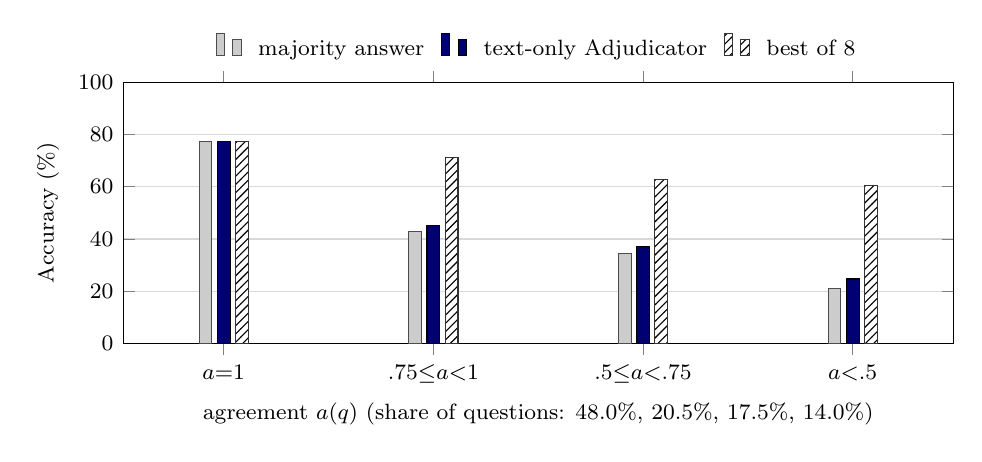
\begin{tikzpicture}
\begin{axis}[
  ybar, bar width=4.6pt, width=\columnwidth, height=4.9cm,
  symbolic x coords={c1,c2,c3,c4},
  xtick=data, xticklabels={$a{=}1$, $.75{\le}a{<}1$, $.5{\le}a{<}.75$, $a{<}.5$}, ymin=0, ymax=100, enlarge x limits=0.16,
  ylabel={Accuracy (\%)}, ylabel style={font=\footnotesize},
  xlabel={agreement $a(q)$ (share of questions: 48.0\%, 20.5\%, 17.5\%, 14.0\%)}, xlabel style={font=\footnotesize},
  tick label style={font=\footnotesize},
  legend style={font=\footnotesize, at={(0.5,1.04)}, anchor=south, legend columns=3, draw=none, column sep=4pt},
  ymajorgrids, grid style={black!15}
]
\addplot[fill=black!20, draw=black!70] coordinates {(c1,77.3) (c2,42.7) (c3,34.3) (c4,21.2)};
\addplot[fill=blue!45!black, draw=black] coordinates {(c1,77.3) (c2,45.2) (c3,37.0) (c4,24.7)};
\addplot[fill=white, draw=black!80, postaction={pattern=north east lines}] coordinates {(c1,77.3) (c2,71.3) (c3,62.7) (c4,60.4)};
\legend{majority answer, text-only Adjudicator, best of 8}
\end{axis}
\end{tikzpicture}
\caption{Accuracy of the majority answer, of the text-only Adjudicator and of the best of the eight candidates (an upper bound) by agreement level, on our 200 questions.}
\label{fig:agreement}
\end{figure}

\vspace{3pt}\noindent\textit{Where the errors are.} Of our 200 questions, 10.5\% have eight identical wrong answers, another 17\% have disagreeing candidates and none of them is correct, and 15.5\% have a correct candidate that DocLens does not return. The first two groups, together 27.5\% of the questions, are errors of evidence retrieval or reading, which no Adjudicator can repair. The Page Navigator of our run recalls 88.4\% of the evidence pages with a precision of 48.7\% and returns 8.6 pages per question. Only the last group, 15.5\% of the questions, is open to a better final decision, and our visual Adjudicator recovers a small part of it.

\vspace{3pt}\noindent\textit{Threshold of the gate.} Table~\ref{tab:tau} shows the text-only gate for every threshold. The accuracy reaches 56.3 at $\tau=0.875$ with 42\% of the calls and stays there at $\tau=1$ with 52\%. We use $\tau=1$ because it needs no tuning, whereas the values near 0.875 were found on the same questions.

\begin{table}[t]
\caption{Accuracy (\%) and Adjudicator rate (\%) of the gate with the text-only Adjudicator for different thresholds $\tau$. $\tau=0$ is majority voting and $\tau>1$ is DocLens.}
\label{tab:tau}
\centering
\footnotesize
\setlength{\tabcolsep}{3.2pt}
\begin{tabular}{@{}lcccccccc@{}}
\toprule
$\tau$ & 0 & .375 & .5 & .625 & .75 & .875 & 1 & $>1$ \\
\midrule
Acc. & 54.8 & 55.3 & 55.3 & 55.3 & 55.8 & 56.3 & 56.3 & 56.3 \\
Adjud. & 0 & 5.5 & 14.0 & 24.5 & 31.5 & 42.0 & 52.0 & 100 \\
\bottomrule
\end{tabular}
\end{table}

\ifextended
\vspace{3pt}\noindent\textit{Additional questions.} We also run DocLens and our method on 400 further questions that do not overlap with the first 200 and were not used to design the method. Table~\ref{tab:extended} shows the result.

\begin{table}[t]
\caption{Accuracy (\%) on additional questions (TBD: to be filled in after the runs).}
\label{tab:extended}
\centering
\footnotesize
\begin{tabular}{@{}lccc@{}}
\toprule
Method & 200 (seed 0) & 400 new & All 600 \\
\midrule
Majority vote & 54.8 & TBD & TBD \\
DocLens & 56.3 & TBD & TBD \\
Gated visual adjudication & 57.3 & TBD & TBD \\
\bottomrule
\end{tabular}
\end{table}
\fi

\section{Conclusion}
\label{sec:conclusion}
We studied the last step of sampling-based document agents, the choice among candidate answers. We gave a formal view of the step, derived the accuracy and cost of an agreement gate, and proposed a visual Adjudicator that checks the candidates against the evidence pages. With Qwen3-VL-8B on 200 MMLongBench-Doc questions, the gate removes 48\% of the Adjudicator calls without a loss of accuracy, and the visual Adjudicator raises the accuracy from 56.3\% to 57.3\%, with the gain on table and figure questions, at 6.7\% more tokens. The agreement of the samples is a good signal of when adjudication is needed: the Adjudicator never helped on unanimous questions and helped by 2.5 to 3.5 points on the others.

The study has limits. The sample has only 200 questions, so the gain of 1.0 point lies within the sampling error, and we designed the visual Adjudicator after looking at the results on the same questions. Our numbers are below the published ones because of the 2$\times$T4 setup and the Qwen answer extractor. With a stricter extraction prompt, DocLens scores 53.6 and vanilla scores 35.8, and the order of these methods does not change. We did not run the visual Adjudicator on every question, so we cannot separate the effect of the gate from the effect of the visual input in that setting, and we tested one backbone only. Most errors come from evidence retrieval and reading, not from the final decision. Future work is a larger evaluation, other backbones, better page recall, and a visual Adjudicator that can abstain.

\section*{Declarations}
\textit{Data availability.} MMLongBench-Doc is available from its authors \cite{ma2024mmlongbench}. The question sample and the saved answers of all runs are available in the repository below.

\textit{Code availability.} The code and the prompts are available at \url{https://github.com/Mariam1543/aqqal123}.

% Funding, Conflict of interest, Ethics approval and consent, Consent for publication, Materials availability and
% Author contribution: add these statements if the venue asks for them (write ``Not applicable'' where they do not apply).


\bibliographystyle{IEEEtran}
\bibliography{references}

\end{document}
